                                                                                                                                                                                                                                                                                                                                                                                                                                                                                                                                                                                                                                                                                                                                                                                                                                                                                                                                                                                                                                                                                                                                                                                                                                                                                                                                                                                                      \begin{frame}
\titlepage
\end{frame}
\begin{frame}
\frametitle{Problem Statement-Triangle Exercise}


\begin{enumerate}[label=(\roman*)]
\item ABC and DBC are two triangles on the same
base BC. If AD intersects BC at O, show that\\
$\frac{ar(ABC)}{ar(DBC)}=\frac{AO}{DO}$\\
\end{enumerate}
\textbf{Soln:}\\

\url{https://github.com/Rajolep/_Geometry/blob/master/figs/triexe.tex}
\begin{figure}
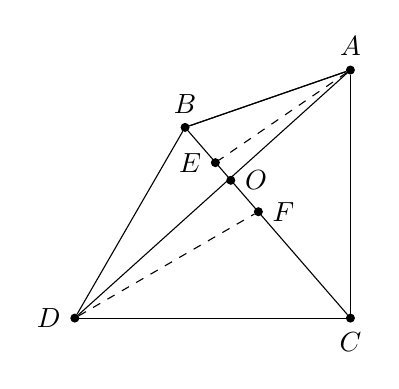
\begin{tikzpicture}
[scale = 0.7,>=stealth,point/.style = {draw, circle, fill = black, inner sep = 1pt}]
\node (A) at (5,4.5)[point,label=above :$A$] {};
\node (D) at (0,0)[point,label=left :$D$] {};
\node (C) at (5,0)[point,label=below :$C$] {};
\node (B) at (2,3.46)[point,label=above :$B$] {};
\node (E) at (2.55,2.82)[point,label=left :$E$] {};
\node (F) at (3.33,1.93)[point,label=right :$F$] {};
\node (O) at (2.83,2.50)[point,label=right :$O$] {};
\draw (D)--(C);
\draw (D)--(A);
\draw (A)--(B);
\draw (C)--(A);
\draw (A)--(B);
\draw (B)--(D);
\draw (B)--(C);
\draw [dashed] (A) -- (E);
\draw [dashed] (D) -- (F);
\tkzMarkRightAngle[draw=red,size=.2](A,E,C)
\tkzMarkRightAngle[draw=red,size=.2](D,F,E)
\end{tikzpicture}
\end{figure}
\end{frame}
\begin{frame}

\begin{itemize}
\item DC=a=4  CA=b=6
\item D=(0,0) \\
\item C=(4,0)\\
\item O=$\frac{(A+D)}{2}$ \\
\item B=(2O$-$C)=B(2.05,5.63)\\
\item A(p,q)\\
\item p=$\frac{a^2+c^2-b^2}{2a}$ q=$\sqrt{c^2-p^2}$\\
\item A(6.05,5.63)\\
\item F=(3.57,1.23)\\
\item E=(2.47,4.40)
\end{itemize}

\end{frame}
\begin{frame}
\begin{figure}
\includegraphics[scale=0.4]{./figs/triexe.eps}
\end{figure}
\url{https://github.com/Rajolep/_Geometry/blob/master/codes/triangle/triangexer.py}
\end{frame}
\begin{frame}
\begin{align*}
AE\perp BC , DF\perp BC\\
Area of \triangle{ABC} = \frac{1}{2}(BC)(AE)\\
Area of \triangle{DBC} = \frac{1}{2}(BC)(DF)\\
\frac{ar\triangle{ABC}}{ar\triangle{DBC}}=\frac{\frac{1}{2}(BC)(AE)}{\frac{1}{2}(BC)(DF)}\\  
\frac{ar\triangle{ABC}}{ar\triangle{DBC}}=\frac{AE}{DF}\\
\frac{AE}{DF}=\frac{AO}{DO}\\
\angle{AEO}=\angle{DFO}..... RA\\
\angle{AEO}=\angle{DOF}..... VOA\\
\triangle{AOE} \sim \triangle{DOF}\\
\frac{AE}{DF}=\frac{AO}{DO}\\
\end{align*}
\end{frame}
\begin{frame}
\begin{align*}
AE=2.407\\
BC=e=9.10294\\
DF=3.4756\\
AO=AE...(1)\\
DO=DF...(2)\\
\end{align*}
From  (1) and  (2)\\
Area of $\triangle{ABC} = \frac{1}{2}(BC)(AE)  = 38.0739$\\
Area of$ \triangle{DBC} = \frac{1}{2}(BC)(DF)  = 38.0739$\\
\end{frame}